\documentclass[10pt]{beamer}
\usetheme{jambro}

\title[]{Macroeconomia I - Comportamento forward-looking e teoria do consumo}
\author[]{Paulo Victor da Fonseca}
\date{18 de abril de 2023}

\hypersetup{
    colorlinks = true,
    urlcolor = teal,
    linkcolor = teal    
}
\usepackage[portuguese]{babel}
\usepackage{subfig}
\usepackage{emoji}
\usepackage{hyperref}

\begin{document}

\begin{frame}[plain]
    \titlepage{
        \begin{center}
            \begin{minipage}{0.8\textwidth}
                \centering
            \end{minipage}
        \end{center}}
\end{frame}

\begin{frame}{Sumário}
    \tableofcontents
\end{frame}

\section{Comportamento forward-looking}
\begin{frame}
    {Comportamento forward-looking}
    \begin{itemize}
        \item Decisões de gastos no presente são influenciadas por \hlight{expectativas} com relação ao futuro\bigskip
        \item Portanto, há um componente \hlight{intertemporal} tanto para decisões de consumo quanto de investimento\bigskip
        \begin{enumerate}
            \item Famílias ajustam consumo corrente baseado em suas expectativas de renda futura: baixa renda corrente mas renda futura esperada elevada pode levar indivíduos a tomar empréstimos no presente, aumentar consumo e pagar dívidas no futuro - \textcolor{blue}{suavização do consumo}\medskip
            \item Decisões das firmas são baseadas em planos de negócios que incluem previsões de demanda futura pelos seus produtos e custos dos insumos. Investimento é intrinsicamente forward-looking dado que custos são incorridos no presente, mas fluxo de benefícios é realizado no futuro
        \end{enumerate}
    \end{itemize}
\end{frame}

\subsection{Valor presente}
\begin{frame}
    {Valor presente}
    \begin{itemize}
        \item O cálculo do \hlight{valor presente} de um fluxo de renda ou lucros futuros pode ser exemplificado pelas decisões de investimento\bigskip
        \item Uma firma maximizadora de lucros realizará projetos de investimento se retorno associado superar custos incorridos\bigskip
        \item Gastos com investimento, tipicamente, precedem retornos que podem ser irregulares e distribuídos ao longo do tempo\bigskip
        \item Lidamos com este fato calculando o \hlight{valor presente} ($V$) do fluxo esperado de lucros $\Pi$ ao longo do tempo
    \end{itemize}
\end{frame}

\begin{frame}
    {Valor presente}
    \begin{itemize}
        \item Com uma taxa de juros de 10\% a.a., se um indivíduo poupa \$100 hoje, receberá \$110 em um ano\bigskip
        \item De outra forma, \$110 no ano seguinte tem o mesmo valor que \$100 hoje, i.e., seu valor presente é \$100\bigskip
        \item De maneira geral, com uma taxa de juros constante e igual a $r$, o valor presente de $X$ unidades monetárias em $n$ anos é igual a $\frac{X}{(1 + r)^n}$ hoje\bigskip
        \item Portanto, o valor presente do fluxo esperado de lucros, $\Pi^e$, de um projeto de investimento com lucros ao longo de $T$ anos é dado por:
        \begin{equation}
            V_t^e = \Pi_t^e + \frac{\Pi_{t+1}^e}{(1 + r)} + \frac{\Pi_{t+2}^e}{(1 + r)^2} + \dots + \frac{\Pi_{t+T}^e}{(1 + r)^T} = \sum_{k = 0}^T \frac{1}{(1 + r)^k}\Pi_{t+k}^e\label{aula7_eq1}
        \end{equation}
    \end{itemize}
\end{frame}

\begin{frame}
    {Valor presente}
    \begin{itemize}
        \item Se custo de máquinas e equipamentos $>$ valor presente do fluxo de lucros, seria mais lucrativo colocar dinheiro no banco ou em títulos (que paguem taxa de juros $r$)\bigskip
        \item Se montante utilizado para aquisição de máquinas e equipamentos é obtido via empréstimos, se o custo superar o valor presente, esta aquisição não seria lucrativa\bigskip
        \item Por outro lado, se o valor presente $>$ custo, então, o investimento será lucrativo e uma firma maximizadora de lucros realizará o plano de investimento
    \end{itemize}
\end{frame}

\begin{frame}
    {Valor presente}
    \begin{itemize}
        \item Mesma lógica para modelar decisões de consumo\bigskip
        \item Futuro influencia decisões de consumo presente: calculamos valor presente do fluxo de renda esperado ao longo do período de vida do consumidor\bigskip
        \item Se assumirmos que indivíduo vive para sempre, o valor presente esperado de sua riqueza ao longo da vida, $\Psi^e$, em $t$ é dado por:
        \begin{equation}
            \Psi_t^e = (1 + r)A_{t-1} + \sum_{k=0}^\infty \frac{1}{(1 + r)^k}y_{t+k}^e\label{aula7_eq2}
        \end{equation}
        \begin{enumerate}
            \item $\sum_{k=0}^\infty \frac{1}{(1 + r)^k}y_{t+k}^e$: valor presente esperado dos rendimentos pós-taxação ao longo da vida\medskip
            \item $(1 + r)A_{t-1}$: recursos disponíveis em $t$ dos ativos mantidos ao final do período anterior
        \end{enumerate}
    \end{itemize}
\end{frame}

\section{Consumo}
\begin{frame}
    {Consumo}
    \begin{itemize}
        \item A renda de um indivíduo flutua ao longo do ciclo de vida\bigskip
        \item Também pode flutuar quando perde emprego, troca de posto de trabalho ou é promovido\bigskip
        \item Indivíduos preferem suavizar flutuações de seus rendimentos em suas decisões de consumo: devem levar em consideração expectativas futuras e ser capazes de tomar empréstimos ou poupar\bigskip
        \item Modelagens de decisões de consumo devem considerar como famílias formam expectativas com relação ao futuro e como poupam ou tomam empréstimos
    \end{itemize}
\end{frame}

\begin{frame}
    {Consumo}
    \begin{itemize}
        \item Desejo de suavizar consumo diante de flutuações de rendimentos é captado pela hipótese de utilidade marginal do consumo decrescente\bigskip
        \item Considere um modelo de 2 períodos\bigskip
        \item Se indivíduo sabe que renda será mais elevada no período seguinte, qual influência sobre decisão de consumo corrente?\bigskip
        \item Considere escolha entre: (i) baixo consumo ($=$ renda) no período 1 e consumo elevado ($=$ renda) no período 2; e (ii) a média dos dois níveis de consumo em cada um dos períodos\bigskip
        \item Se $U_{CC}(\bullet) < 0$, consumo maior sempre aumenta utilidade, mas aumentos sucessivos trazem benefícios cada vez menores\bigskip
        \item Portanto, famílias escolherão segunda opção: consumir média nos dois períodos oferece utilidade maior que primeira opção
    \end{itemize}
\end{frame}

\section{Hipótese da renda permanente}
\begin{frame}
    {Hipótese da renda permanente}
    \begin{itemize}
        \item A \hlight{hipótese da renda permanente} afirma que indivíduos escolhem, de maneira ótima, o quanto consumir de maneira a alocar seus recursos ao longo de seus ciclos de vida\bigskip
        \item Teoria desenvolvida, inicialmente, por Modigliani e Brumberg (1954)\bigskip
        \item Popularizada por Milton Friedman com o livro \emph{A theory of the consumption function} - 1957
    \end{itemize}
\end{frame}

\begin{frame}{Hipótese da renda permanente}
    \begin{figure}
        \centering
        \subfloat[\href{https://en.wikipedia.org/wiki/Franco_Modigliani}{Franco Modigliani (1918 - 2013)}\label{aula7_fig1}]{\href{https://en.wikipedia.org/wiki/Franco_Modigliani}{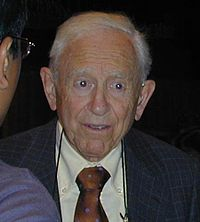
\includegraphics[width=0.3\textwidth]{./figures/aula7_fig1.jpg}}} \qquad
        \subfloat[\href{https://en.wikipedia.org/wiki/Milton_Friedman}{Milton Friedman (1912 - 2006)}\label{aula7_fig2}]{\href{https://en.wikipedia.org/wiki/Milton_Friedman}{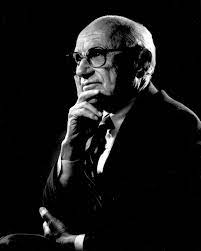
\includegraphics[width=0.27\textwidth]{./figures/aula7_fig2.jpeg}}}        
        %\caption{Bibliografia do curso}
        \label{aula7_fig1pih}
    \end{figure}
\end{frame}

\begin{frame}
    {Hipótese da renda permanente}
    \begin{itemize}
        \item Recursos de um indivíduo: ativos + renda presente e futura\bigskip
        \item A alocação de recursos ao longo do ciclo de vida é decisão \emph{forward-looking} e dependerá da taxa de juros, valor dos ativos e expectativas acerca de rendimentos e tributação futuros\bigskip
        \item Hipótese da renda permanente: trajetória de consumo ótima é suave quando comparada à da renda\bigskip
        \item E.g.: no início da vida laboral, rendimentos são baixos e, então, indivíduos tomam empréstimos para consumir mais\bigskip
        \item Quando renda aumenta, consumo é mantido constante e excedente de rendimentos é utilizado para pagar dívidas e poupar para aposentadoria\bigskip
        \item Na aposentadoria, rendimentos caem e, então, agentes retiram de suas poupanças
    \end{itemize}
\end{frame}

\begin{frame}
    {Hipótese da renda permanente}
    \begin{figure}
        \centering
        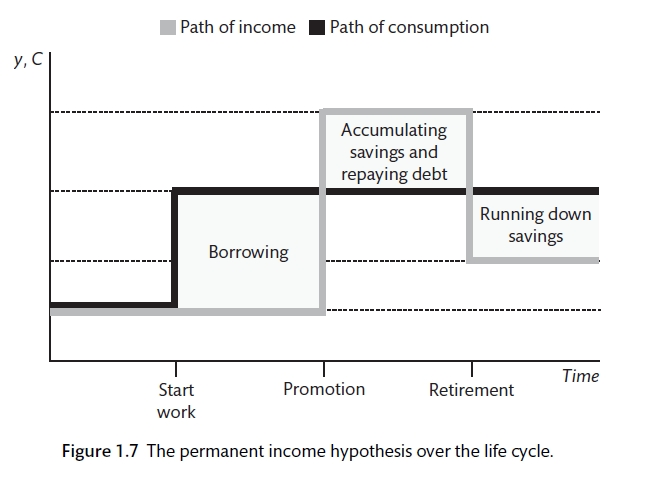
\includegraphics[width=0.6\textwidth]{./figures/aula7_fig3.jpg}
        \caption{Hipótese da renda permanente ao longo do ciclo de vida. Fonte: Carlin e Soskice (2015)}
    \end{figure}
\end{frame}

\begin{frame}
    {Hipótese da renda permanente}
    \begin{itemize}
        \item \hlight{Indivíduo irá contrair empréstimos e poupar para assegurar suavização da trajetória de consumo ao longo do ciclo de vida}\bigskip
        \item Analogamente, ao longo do ciclo de negócios, se indivíduo torna-se desempregado, contrai empréstimos para sustentar nível de consumo durante período de desemprego\bigskip
        \item A política fiscal tem papel relevante na suavizaçãod e consumo ao prover benefícios como seguro-desemprego (estabilizador automático)\bigskip
        \item HRP $\neq$ teoria de consumo Keynesiana (não há consideração explícita a respeito do futuro)
    \end{itemize}
\end{frame}

\begin{frame}
    {Hipótese da renda permanente}
    \begin{itemize}
        \item HRP: bom ponto inicial para pensarmos em escolha intertemporal e decisões de consumo \emph{forward-looking}\bigskip
        \item Como rendimentos oscilam ao longo do ciclo de vida, indivíduos contraem empréstimos/poupam para atingir objetivo de suavizar consumo\bigskip
        \item Mas é preferível uma trajetória de consumo constante em cada período, ou uma trajetória ascendente ou descendente de consumo?\bigskip
        \item Depende da relação entre taxa de juros sobre empréstimos e poupança e a taxa de trade-off entre consumo futuro e consumo presente do invidíduo\bigskip
        \item Esta última é a taxa de desconto subjetiva, $\rho$ - medida do grau de impaciência
    \end{itemize}
\end{frame}

\begin{frame}
    {Hipótese da renda permanente}
    \begin{itemize}
        \item Família escolhe trajetória de consumo que maximiza valor presente da utilidade (derivada do consumo) ao longo do ciclo de vida sujeito à restrição orçamentária intertemporal\bigskip
        \item Valor presente da utilidade intertemporal:
        \begin{equation}
            V_t^e = \sum_{k = 0}^\infty \frac{1}{(1 + \rho)^k}U(C_{t + k})
            \label{aula7_eq3}
        \end{equation}
        \item Utilidade de consumo descontada para período corrente pela taxa subjetiva de desconto intertemporal, $\rho$\bigskip
        \item Consumo futuro terá utilidade menor para consumidores mais impacientes\bigskip
        \item O valor presente esperado da riqueza total ao longo da vida é:
        \begin{equation}
            \Psi_t^e = (1 + r)A_{t-1} + \sum_{k=0}^\infty \frac{1}{(1 + r)^k}y_{t+k}^e
            \label{aula7_eq4} 
        \end{equation}
    \end{itemize}
\end{frame}

\begin{frame}
    {Hipótese da renda permanente}
    \begin{itemize}
        \item Restrição orçamentária pode ser escrita como:
        \begin{equation}
            A_t + C_t = (1 + r)A_{t-1} + y_t
            \label{aula7_eq5}
        \end{equation}
        \item Resolvendo problema de otimização dinâmica, obtemos a \hlight{equação de Euler}:
        \begin{equation}
            \tikz[tstyle]{\node[nstyle](node0){$U'(C_t)$}} = \tikz[tstyle]{\node[nstyle](node1){$\frac{1 + r}{1 + \rho}U'(C_{t+1}^e)$}}
            \label{aula7_eq6}
        \end{equation}
        \begin{tikzpicture}[tpstyle]
			\node[pencil,very thick, brick, draw, minimum height=0.8cm, minimum width=1.2cm] (box0) at (node0) {};
            \node[pencil,very thick,draw, minimum height=0.8cm, minimum width=2cm] (box1) at (node1) {};
		\end{tikzpicture}
        \item Eq. de Euler nos diz valor ótimo de $C_t$ em relação a $C_{t+1}^e$\bigskip
        \item No período corrente, indivíduo compara ganhos de consumir mais neste período com a perda descontada de consumir menos no período seguinte
        \begin{tikzpicture}[tpstyle]
			\draw[arrow, brick, ->] ([yshift=2pt]box0.west) to[bend left] +(-0.4,0.1) node[anchor=east,opacity=1] {\hand Ganho de consumir unidade adicional};
            \draw[arrow,->] ([yshift=2pt]box1.south west) to[bend right] +(+0.1,-0.3) node[anchor=west,opacity=1] {\hand VP subjetivo da perda de utilidade próx. período};
		\end{tikzpicture}
    \end{itemize}
\end{frame}

\begin{frame}
    {Hipótese da renda permanente}
    \begin{itemize}
        \item No próx. período, a renda do consumidor terá sido reduzida em uma magnitude $(1 + r)$, multiplicada pela utilidade marginal do consumo e pelo fator de impaciência\bigskip
        \item O consumidor não consegue atingir utilidade mais elevada do que quando o ganho de consumir uma unidade adicional no período corrente é exatamente equivalente ao valor presente subjetivo de perda de utilidade de consumir uma unidade adicional a menos no período seguinte
    \end{itemize}
\end{frame}

\begin{frame}
    {Hipótese da renda permanente}
    \begin{itemize}
        \item Eq. de Euler para utilidade logarítmica:
        \begin{eqnarray}
            \frac{1}{C_t} &=& \left(\frac{1 + r}{1 + \rho}\right) \frac{1}{C_{t+1}^e} \nonumber \\
            C_t &=& \left(\frac{1 + \rho}{1 + r}\right)C_{t+1}^e\label{aula7_eq7}
        \end{eqnarray}
        \item \hlight{Regra Keynes-Ramsey}: consumo crescente quando juro real $r$ maior que taxa de desconto $\rho$\bigskip        
        \item Se $r < \rho$, trajetória de consumo será decrescente
    \end{itemize}
\end{frame}

\begin{frame}
    {Hipótese da renda permanente}
    \begin{itemize}
        \item Intuição mais clara se $\rho = r$\bigskip
        \item Família obtem mesmo retorno (objetivo) ao poupar, $r$, que sua disposição (subjetiva) de trocar consumo presente por consumo futuro, $\rho$\bigskip
        \item Com $r = \rho$, \hlight{indivíduo prefere um nível constante de consumo em cada período do tempo}: $C_t = C_{t+1}^e$\bigskip
        \item O ponto crucial é que, independente de qual padrão de consumo seja prevalente, ele é independente das variações temporárias (período a período) de renda
    \end{itemize}
\end{frame}

\begin{frame}
    {Hipótese da renda permanente}
    \begin{itemize}
        \item Análises posteriores: assumiremos $\rho = r$\bigskip
        \item Para implementar plano ótimo de suavização do consumo ao longo do ciclo de vida, dada a renda de cada período, indivíduo deve poupar ou tomar empréstimo que for necessário para manter consumo constante\bigskip
        \item Se renda corrente está acima da renda permanente, indivíduo poupará\bigskip
        \item Caso contrário, toma emprestado
    \end{itemize}
\end{frame}

\begin{frame}
    {Hipótese da renda permanente}
    \begin{itemize}
        \item Se $\rho = r$, consumo em cada período é dado por:
        \begin{equation}
            C_t = \frac{r}{1 + r}\Psi_t^e\label{aula7_eq8}
        \end{equation}
        \item Intuição: consumidor poupa e toma empréstimo para obter trajetória de consumo perfeitamente suave (em expectativas)\bigskip
        \item A quantidade consumida em cada período é dada pelo valor de anuidade da riqueza esperada ao longo da vida: \hlight{renda permanente}\bigskip
        \item Indivíduo consome sua renda permanente e (\ref{aula7_eq8}) assegura que, em expectativa, o faz para sempre\bigskip
        \item Consumo permanece constante, a não ser que $\Psi_t^e$ se altere
    \end{itemize}
\end{frame}


\begin{frame}{\emoji{books} Bibliografia}
    \begin{itemize}
        \item BLANCHARD, O. Macroeconomia. 7.ed. São Paulo: Pearson Education do Brasil, 2017\medskip        
        \item CARLIN, W.; SOSKICE, D. Macroeconomics: Institutions, instability, and the financial system. Oxford, UK: Oxford University Press, 2015\medskip
        \item DORNBUSCH, R.; FISCHER, S.; STARTZ, R. Macroeconomia. 11.ed. Porto Alegre: AMGH, 2013. Disponível em: \href{https://app.minhabiblioteca.com.br/books/9788580551853}{app.minhabiblioteca.com.br/books/9788580551853}\medskip
        \item MISHKIN, F.S. The economics of money, banking, and financial markets. 11.ed. Pearson Education Limited, England, 2016.
    \end{itemize}
\end{frame}
\end{document}